% AUTO-GENERATED durch diagram_generator (A2/m3v2, Working-Set-Sweep-Kurve; z=ns_per_op; lang=de)
% Eine Kurve je gesweepter Achsen-Auspraegung; X=working_set_n (log2), Y=ns_per_op (nearest-rank-Median, nur two_phase_valid).
\begin{figure}[!htbp]
\centering
\resizebox{\textwidth}{!}{%
\begin{tikzpicture}
\begin{axis}[
    width=0.7800\textwidth,
    height=0.4000\textheight,
    scale only axis,
    title={Working-Set-Sweep: Gesamt-Latenz (ns/op)},
    xlabel={Arbeitsmenge n (Schluessel)},
    ylabel={Gesamt-Latenz (ns/op)},
    grid=both,
    enlargelimits=0.05,
    xmode=log,
    log basis x=2,
    % P1b: nur EIN gemessener working_set_n -> Achse explizit auf eine Oktave geweitet
    % (sonst xmin==xmax -> "Axis range for axis x is approximately empty"). Nur die ACHSE.
    xmin=2048.0000, xmax=8192.0000,
    legend pos=north west,
    legend style={font=\tiny},
    mark size=2pt,
]
\addplot+[mark=*] coordinates {
    (4096,671.5320)
};
\addlegendentry{k\_ary}
\end{axis}
\end{tikzpicture}
}%
\caption{Working-Set-Sweep: Gesamt-Latenz (ns/op)}
\end{figure}
